\documentclass[tikz,border=4pt]{standalone}
% Shared setup for the foundation-model diagrams, in the AFRICAST palette
\usepackage{fontspec}
\usepackage[sfdefault]{FiraSans}
\usepackage{amsmath}
\usepackage{unicode-math}
\setmathfont{Fira Math}
\usetikzlibrary{arrows.meta}
\definecolor{ink}{HTML}{1F2A36}
\definecolor{MonashBlue}{HTML}{3B75AC}
\definecolor{Orange}{HTML}{B5570F}
\color{ink}
\tikzset{every picture/.style={draw=ink,>=stealth}}
\hyphenpenalty=10000
\exhyphenpenalty=10000

\begin{document}
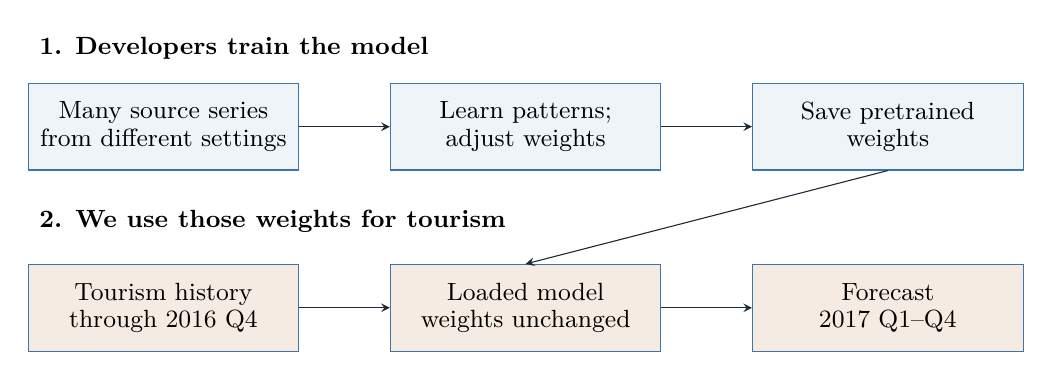
\begin{tikzpicture}[>=stealth,every node/.style={font=\fontsize{9}{10}\selectfont,align=center},
box/.style={draw=MonashBlue,fill=MonashBlue!8,text width=3.2cm,minimum height=1.1cm}]
\node[anchor=west,font=\fontsize{9}{10}\selectfont\bfseries] at (-1.7,1) {1. Developers train the model};
\node[box] (s) at (0,0) {Many source series\\from different settings};
\node[box] (p) at (4.6,0) {Learn patterns;\\adjust weights};
\node[box] (m) at (9.2,0) {Save pretrained\\weights};
\node[anchor=west,font=\fontsize{9}{10}\selectfont\bfseries] at (-1.7,-1.2) {2. We use those weights for tourism};
\node[box,fill=Orange!12] (t) at (0,-2.3) {Tourism history\\through 2016 Q4};
\node[box,fill=Orange!12] (i) at (4.6,-2.3) {Loaded model\\weights unchanged};
\node[box,fill=Orange!12] (o) at (9.2,-2.3) {Forecast\\2017 Q1--Q4};
\draw[->](s)--(p);\draw[->](p)--(m);
\draw[->](t)--(i);\draw[->](m.south)--(i.north);\draw[->](i)--(o);
\end{tikzpicture}
\end{document}
